% ----------------------
  \chapter{Marco Teórico} 
% ----------------------
\label{C:MarcoTeórico}

En este  capítulo se dará una breve descripción teórica de los conceptos relevantes de la domótica, enfatizando conceptos y especificaciones de en la forma en la que se va a desarrollar este proyecto.

%%%------------------------------------------
\section{Domótica}
%%%------------------------------------------
La domótica, dicho en muy pocas palabras, es la instalación e integración de varias redes y dispositivos electrónicos en el hogar, que permiten la automatización de actividades cotidianas y el control local o remoto de la vivienda, o del edificio inteligente \cite{Madrid2007}.

Un sistema domótico es capaz de recoger información proveniente de unos sensores o entradas, procesarla y emitir órdenes a unos actuadores o salidas. El sistema puede acceder a redes exteriores de comunicación o información. La domótica permite dar respuesta a los requerimientos que plantean estos cambios sociales y las nuevas tendencias de nuestra forma de vida, facilitando el diseño de casas y hogares más humanos, más personales, polifuncionales y flexibles. 

Inicialmente, una instalación domótica usaba sensores y actuadores que se unían a un controlador o PLC (Programmable Logic Controller, por sus siglas en inglés) que se encargaba de realizar las tarea de una vivienda, pero este sistema era poco flexible y muy costoso. Pero con el surgimiento de la electrónica y del internet, ahora en el mercado existen una gran cantidad de componentes y protocolos que facilitan la conexión de varios dispositivos, vía ethernet o Wi-Fi. 

En la figura \ref{F:domo}, se ejemplifica mejor el concepto de un sistema domótico.

\begin{figure}[H]
\centering
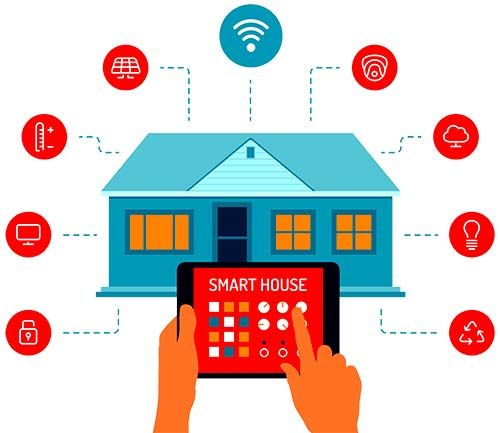
\includegraphics[width=0.8\textwidth]{./imagenes/teoria/domo.jpg} 
\caption{Sistema domótico comercial \cite{Madrid2007}.}
\label{F:domo}
\end{figure}

En la actualidad, han surgido instaladores, constructores, proyectistas, arquitectos, productores y diseñadores que han adquirido una rápida familiarización con esta tecnología  y las posibilidades que ofrecen los dispositivos, por lo que tienen el conocimiento necesario para incorporarlos y ofrecer distintos productos, en un mercado que está incrementado exponencialmente su competitividad e ingresos.
%%%------------------------------------------
\subsection{Ventajas y desventajas de un sistema domótico}
%%%------------------------------------------

Según \cite{Madrid2007}, algunas de las ventajas de un sistema de este tipo son:

\begin{itemize}
\item \textbf{Climatización y consumo energético}: se puede programar el encendido y apagado de aparatos electrónicos y luces, además de usan medidores de energía en tiempo real que informe el consumo al usuario.
\item \textbf{Entretenimiento y confort}: permite conectar el internet a los componentes de la casa, concepto que esta en tendencia con el Internet de las cosas (IoT, \textit{Internet of Things}, por sus siglas en inglés), por lo que se facilita el uso de los componentes del hogar.
\item \textbf{Seguridad}: configuración de procedimientos de avisos en caso de intrusión o avería, instalación de cámaras y micrófonos, control de acceso a la vivienda, entre otros.
\item \textbf{Comunicación}: debido al uso de redes de internet se puede tener un control remoto y tener los datos del estado del hogar desde cualquier parte.
\end{itemize}

Además algunas de las desventajas descritas en \cite{Madrid2007}, son:
\begin{itemize}
\item \textbf{Inversión inicial}: todavía resulta muy caro ya que hay que cablear toda la casa.
\item \textbf{Casas nuevas}: estos sistemas están tienen relativamente mayor exitoso en casas, ya que, en las casa viejas y que no fueron diseñadas para esta tecnología, el costo inicial se incrementa aún más. 
\item \textbf{Problemas de seguridad}: si se usa sistema domótico con control por medio de una red remota, como lo son la mayoría de los que se ofrecen comercialmente, se pueden presentar problemas de seguridad y hackeo del sistema.
\item \textbf{Falta de normativas}: debido al reciente auge de está tecnología, en muchos países, existen pocas normas que regulan la instalación de estos sistemas y no se tienen procedimientos de instalación y mantenimiento que garantice la seguridad de los ocupantes de una vivienda con un sistema domótico.
\end{itemize}

%%%------------------------------------------
\section{Servidor web}
%%%------------------------------------------

En términos sencillos un servidor web es un programa diseñado para permitir la interacción entre ordenadores.

Suele funcionar permaneciendo a la espera de peticiones. Cuando las recibe responde a ellas transfiriendo documentos de tipo hipertexto, Para ello implementa el protocolo HTTP (\textit{HyperText Transfer Protocol}, por sus siglas en inglés). En la figura \ref{F:peticion}, se ejemplifica el concepto de peticiones en un servidor web.

\begin{figure}[H]
\centering
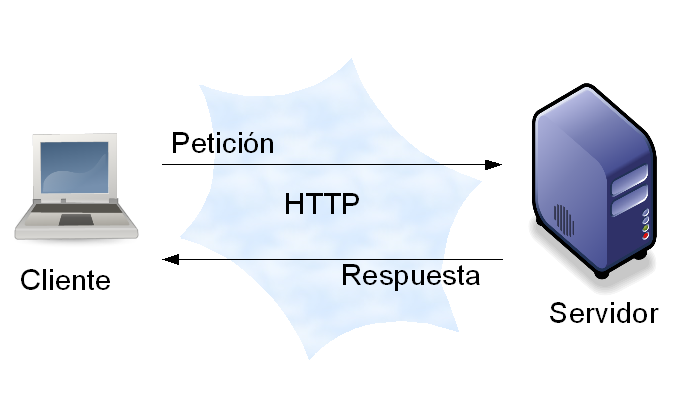
\includegraphics[width=0.55\textwidth]{./imagenes/teoria/peticion.png} 
\caption{Petición en un servidor web.}
\label{F:peticion}
\end{figure}

En donde el servidor y el cliente se encargan de:

\begin{itemize}
\item \textbf{Servidor}:
  \begin{enumerate}
  \item Espera las peticiones
  \item Envía archivos
  \item Ejecuta CGIs (en respuesta a las peticiones) y envía los resultados
  \item Establece conexión a Sistemas de Bases de Datos
  \item Actúa de puerta de enlace para servicios como el correo, ftp, etc
  \end{enumerate}
\item \textbf{Cliente}:
	\begin{enumerate}
    \item Realiza las peticiones
    \item Interpreta el código HTML que recibe
    \item Arranca aplicaciones externas.
    \item Controla aspectos del formato del documento.
	\end{enumerate}
\end{itemize}

Además es importante conocer a cerca de los requisitos mínimos para la implementación de un servidor web, los cuales según \cite{Sanchez2018} son:
\begin{itemize}
\item \textbf{Hardware}: Un ordenador tipo PC de nivel básico (2010-Pentium, 1 Gb RAM, 20 Gb HD)
\item \textbf{Software}: Programas específicos, programas para ejecutar aplicaciones, herramientas de desarrollo
\item \textbf{Conectividad}: Ordenador conectado a internet y ejecutando TCP/IP
\end{itemize}
%%%------------------------------------------
\subsection{Servidor web local}
%%%------------------------------------------

Un servidor web local es aquel que reside en una red local al equipo de referencia. El servidor web local puede estar instalado en cualquiera de los equipos que forman parte de una red local. Es por tanto obvio, que todos los servidores web, son locales a la red local en la que se encuentran, o como mínimo, locales al sistema en el que están instalados. 

En la figura \ref{F:RED}, se muestra una configuración típica de una red local, en este proyecto se van conectar los componentes electrónicos tipo Sonoff por medio de conexión Wi-Fi, al igual que componentes por ethernet, como cámaras. 

\begin{figure}[H]
\centering
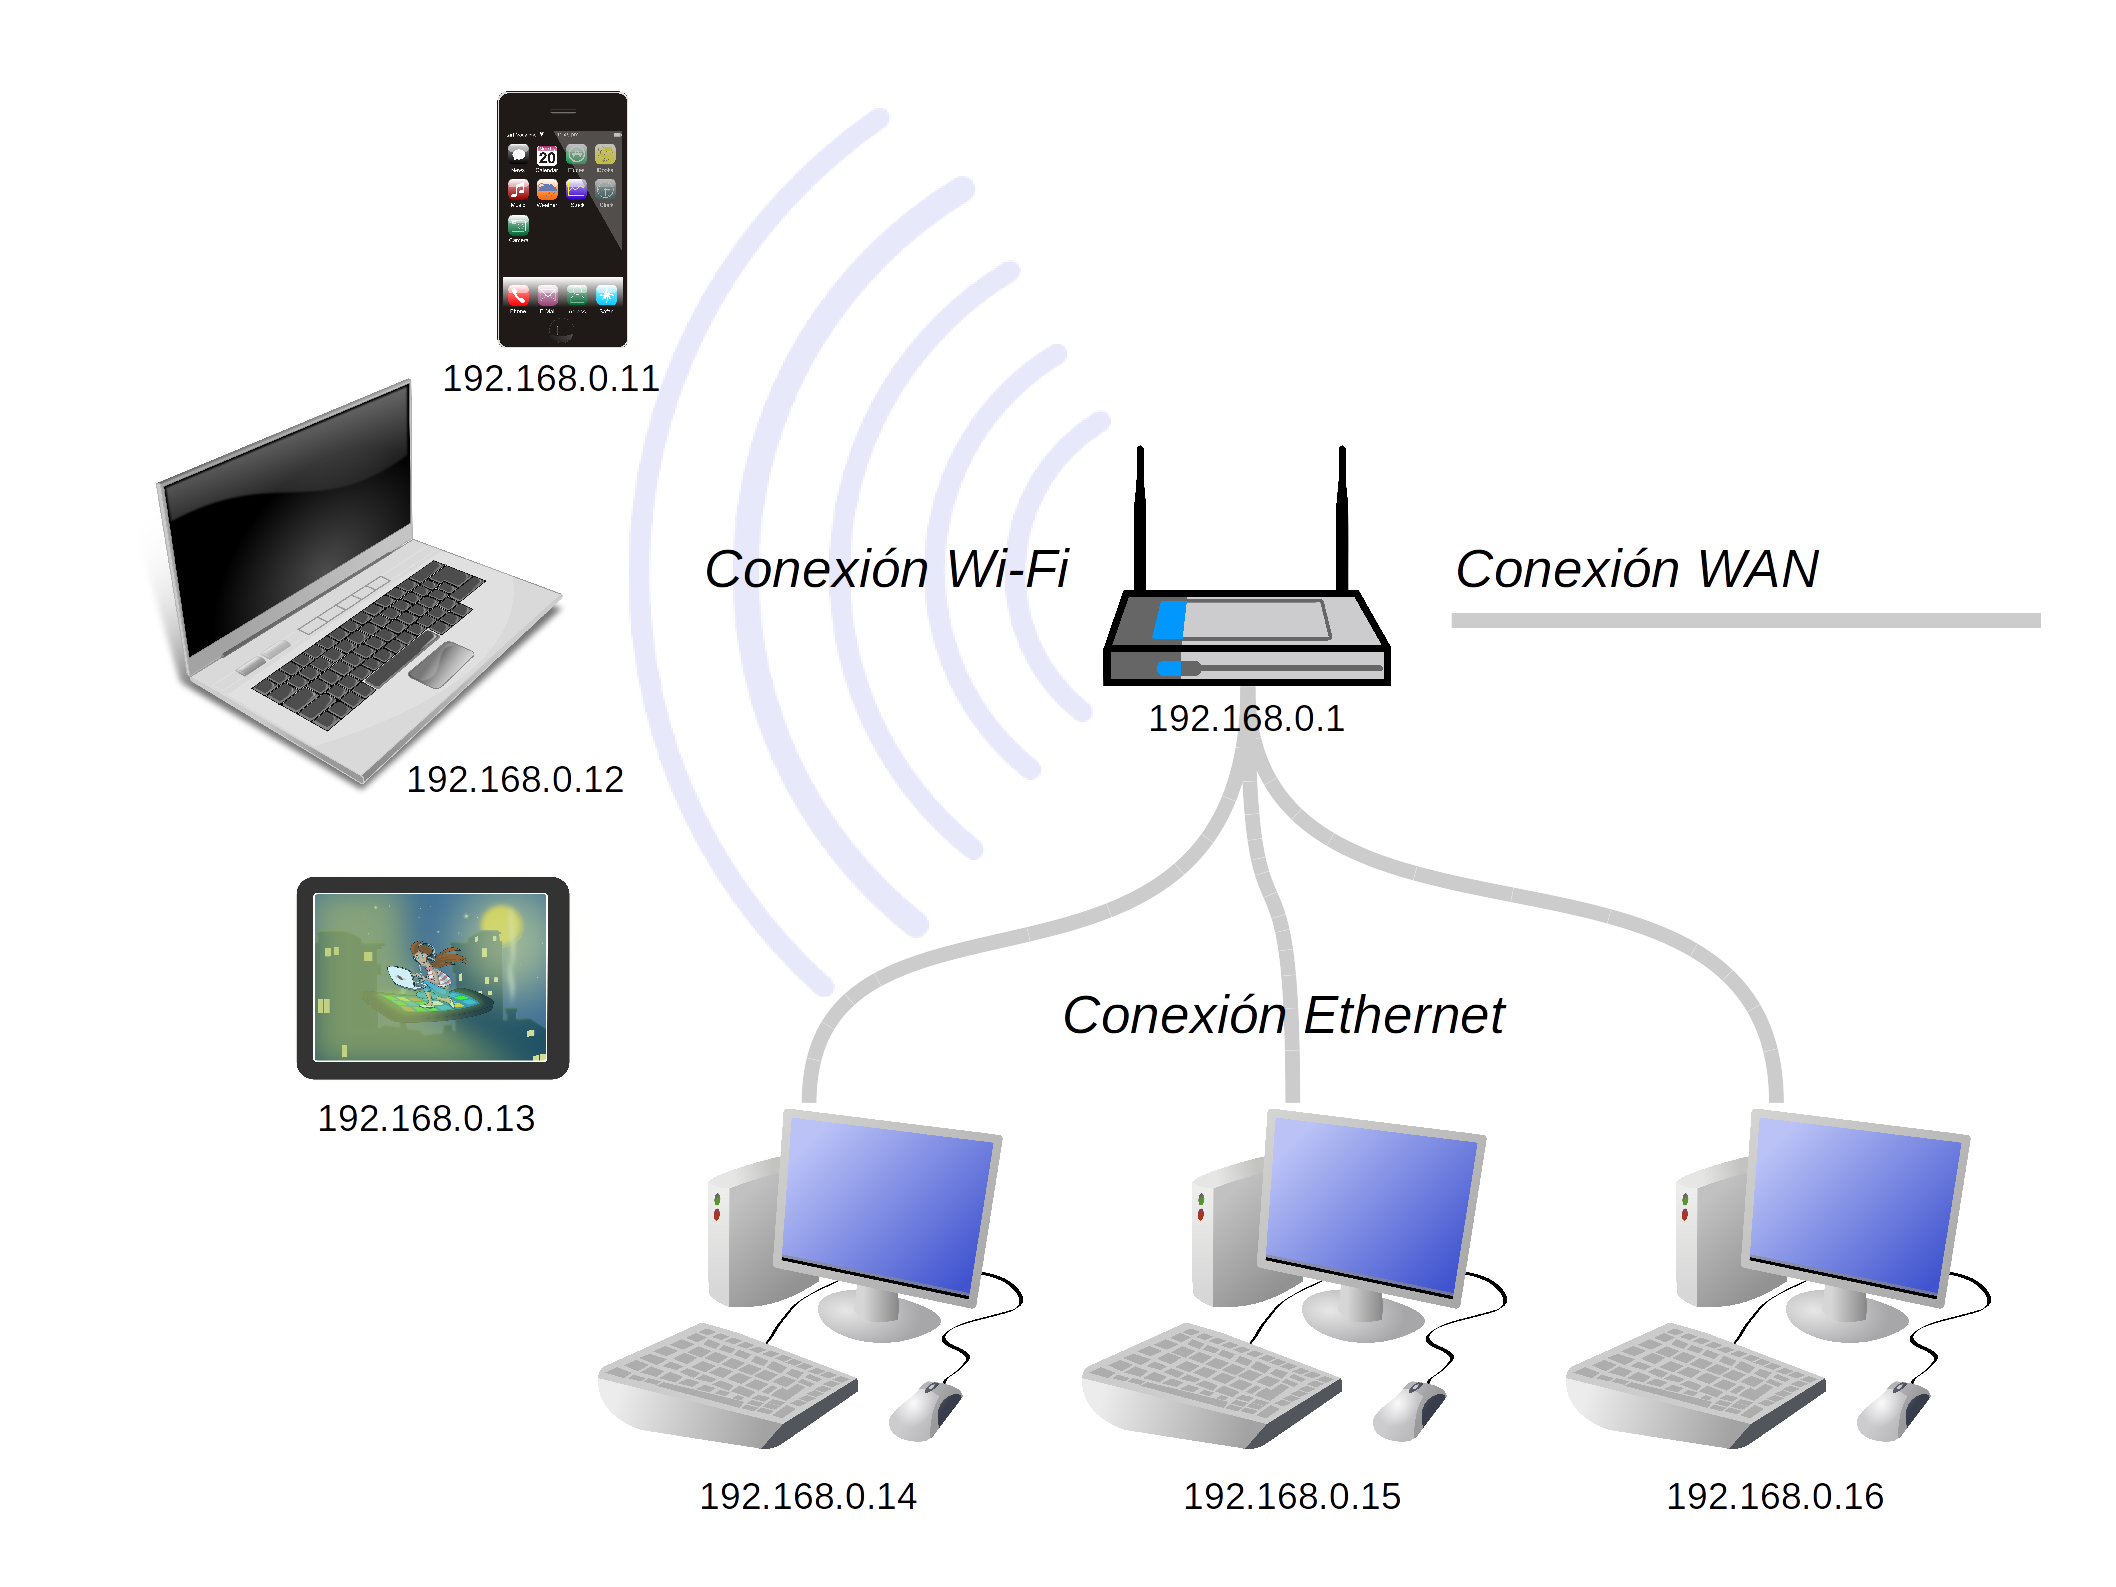
\includegraphics[width=0.8\textwidth]{./imagenes/teoria/red_local.png} 
\caption{Red local con router inalámbrico \cite{Sanchez2018}.}
\label{F:RED}
\end{figure}

Existen numerosas aplicaciones que facilitan la instalación automática de servidores web Apache y aplicaciones adicionales como MySQL y PHP (entre otros), de forma conjunta, como XAMPP, JAMP o EasyPHP. Estas aplicaciones reciben el nombre de LAMP cuando se instalan en plataformas Linux, WAMP en sistemas Windows y MAMP en sistemas Apple Macintosh.

Algunos servidores web importantes son:

\begin{itemize}
\item Nginx
\item Apache
\item Internet Information Services (IIS)
\item Cherokee
\item Tomcat
\end{itemize}

Según \cite{Sanchez2018}, entre las ventajas de un servidor web local se encuentran:

\begin{itemize}
\item Seguridad, ya que, los que acceden al servidor son los equipos conectados a una red local. 
\item Se puede hacer todo tipo pruebas a nuestro sitio sin temor a estropear el sitio, al fin y al cabo, para eso sirve el localhost.
\item No es necesario contratar un dominio (dirección) ya que es 127.0.0.1 y el disco duro funciona como el hosting (y por así decirlo es ilimitado).
\item Teniendo el sitio montado en internet, se puede tener también el localhost como respaldo.
\item Logra minimizar el número de credenciales dentro de la red.
\item Es escalable, por lo que se puede cambiar el tamaño del servidor local fácilmente en el caso de ser necesario.
\end{itemize}

Entre las principales desventajas se encuentran \cite{Sanchez2018}:
\begin{itemize}
\item Es necesario tener una computadora conectada para poder mantener el servidor local.
\item No se puede respaldar la información.
\item Alto consumo de energía y baterías limitadas en caso de fallos de luz
\item Se puede centralizar la gestión de los usuarios y las contraseñas.
\end{itemize}

%%%------------------------------------------
\subsubsection{Nginx}
%%%------------------------------------------

Es un software libre y de código abierto, licenciado bajo la Licencia BSD simplificada; también existe una versión comercial distribuida bajo el nombre de nginx plus. Es multiplataforma, por lo que corre en sistemas tipo Unix (GNU/Linux, BSD, Solaris, Mac OS X, etc.) y Windows.

\begin{figure}[H]
\centering

\includegraphics[width=0.3\textwidth]{./imagenes/teoria/nginz.png} 
\caption{Logo de la marca comercial Nginx.}
\label{F:NGINX}
\end{figure}

%%%------------------------------------------
\subsubsection{Apache}
%%%------------------------------------------
Apache es posiblemente el servidor Web más utilizado en el mundo. Todas las distribuciones Linux cuentan con un servidor Apache integrado en la propia distribución por lo cual solamente hay que seleccionar la opción de instalar el servidor para que éste quede instalado y funcional \cite{Apache2018}.

\begin{figure}[H]
\centering

\includegraphics[width=0.35\textwidth]{./imagenes/teoria/apache.png} 
\caption{Logo de la marca comercial Apache.}
\label{F:APACHE}
\end{figure}

La ventaja de estos dos software, es que se encuentran como licencia libre, lo que facilita la implementación de un servidor local en un dispositivo que corra bajo una distribución GNU/Linux. 


%%%------------------------------------------
\section{Componentes electrónicos Sonoff}
%%%------------------------------------------
El fabricante de estos producto es ITEAD, el cuál se especializa en el desarrollo y fabricación de hardware y productos para el hogar inteligente. Ubicada en Shenzhen, el mercado electrónico más grande de China y la cadena de suministro electrónico más integrada del mundo, lo que permite ofrecer productos innovadores de alta calidad a bajo costo \cite{Sonoff2018}. En la figura \ref{F:sonoff}, se puede ver un ejemplo de uso de estos componentes y como es que se ve una posible instalación de este sistema.

\begin{figure}[H]
\centering
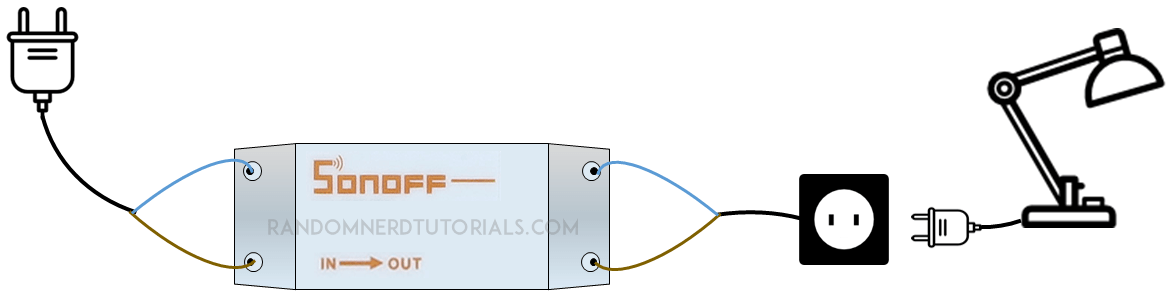
\includegraphics[width=\textwidth]{./imagenes/teoria/SONOFF_circuit.png} 
\caption{Ejemplo de componente domótico \cite{Sonoff2018}.}
\label{F:sonoff}
\end{figure}

Entre las ventajas de estos componentes, es el precio, que ronda entre \$4 - \$20, por lo que son relativamente baratos. Además, como se mencionó en el capítulo anterior, una de las principales ventajas de estos componentes es que permiten la ingeniería inversa. Este concepto consiste en recuperar el diseño de una aplicación o producto a del partir del código o diagramas que ayudan a entender el funcionamiento del componente. El objetivo de la ingeniería inversa es obtener información a partir de un producto accesible al público, con el fin de determinar de qué está hecho, qué lo hace funcionar y cómo fue fabricado. Está característica en lo componentes Sonoff es de vital importancia, ya que, nos permite editar la configuración por defecto de los componentes y adaptarlos para que se comporten de una manera distinta, en nuestro caso esta configuración se hará para realizar la conexión a una red local. 
 
Existen una gran variedad de componentes de esta compañía, a continuación en la tabla \ref{T:Sonoff}, se muestran algunas de las características básicas de cada uno de los componentes Sonoff.

\begin{table}[H]
\centering
\caption{Descripción de los componentes electrónicos Sonoff \cite{Sonoff2018}.} \label{T:Sonoff}
\begin{tabular}{ | >{\centering\arraybackslash}m{2.5cm} | >{\centering\arraybackslash}m{12cm}  | }
    \hline
    \cellcolor{cl} \textbf{Componente} & \cellcolor{cl} \textbf{Funcionamiento}  \\
    \hline
    \hline
    Sonoff Basic & Es un interruptor con conexión Wi-Fi, que se puede programar para que funcione en horas específicas, con operación de \SI{90}{\volt} - \SI{250}{\volt} en AC y capacidad de corriente máxima de \SI{10}{A}.\\ \hline
    Sonoff RF & Cumple con las mismas funciones que el Sonoff Basic, con la diferencia de que se puede utilizar por medio de una infrarroja de \SI{433}{MHz}. \\ \hline
    Sonoff TH10/TH16 & Permite medir la temperatura y la humedad, haciendo uso de sensores de alta precisión.  \\ \hline
    Sonoff Dual & Cumple con funciones similares al Sonoff Basic, con la diferencia de que se pueden utilizar dos cargas y manejarse de manera independiente cada una de ellas. \\ \hline
    Sonoff Pow & Permite el monitoreo del consumo de energía en tiempo real, con operación de \SI{90}{\volt} - \SI{250}{\volt} en AC, capacidad de corriente máxima de \SI{10}{A} y de potencia de \SI{3500}{W}.\\ \hline
    Sonoff 4CH & Básicamente son 4 relés con monitoreo del consumo de energía y que se pueden programar los horarios de operación de los componentes, con operación de \SI{90}{\volt} - \SI{250}{\volt} en AC, capacidad de corriente máxima de \SI{10}{A} y de potencia máxima de \SI{2200}{W}. \\ \hline
    Sonoff G1 & Cumple con las mismas funciones que el Sonoff Basic, con la diferencia de que se puede utilizar por medio de GPRS al conectarle una tarjeta SIM, lo que lo hace ideal para aplicaciones en el área agrícola o en jardines.  \\ \hline 
    Sonoff Pow R2 & Está versión permite monitorear en tiempo real no solo el consumo de energía, sino la tensión y la corriente, además se puede programar para que actué como protección a sobrecargara al poder configurar un valor máximo de carga y se puede generar un registro de los datos.  \\ \hline
    Sonoff 4CH PRO & Similar a la versión 4CH, pero con capacidad de ser utilizado con una señal infrarroja de \SI{433}{MHz} y bloque de los relés.   \\ 
    \hline
\end{tabular}
\end{table}

En la figura \ref{F:PRODUCTS}, se puede observar el diseño físico de cada uno de los componentes descritos en la tabla anterior.

\begin{figure}[H]
\centering
\begin{tabular}{c c c}

\subfloat[Basic]
{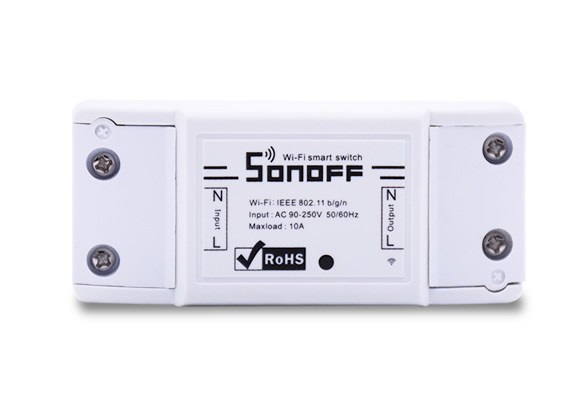
\includegraphics[width=0.33\textwidth]{./imagenes/teoria/BASIC.jpg}}
&
\subfloat[RF]{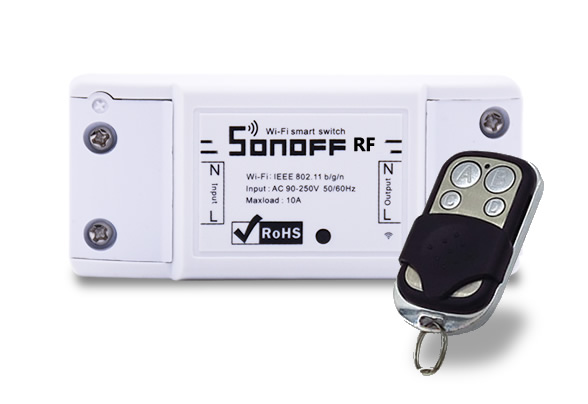
\includegraphics[width=0.33\textwidth]{./imagenes/teoria/RF.jpg} }
&
\subfloat[TH10/TH16]{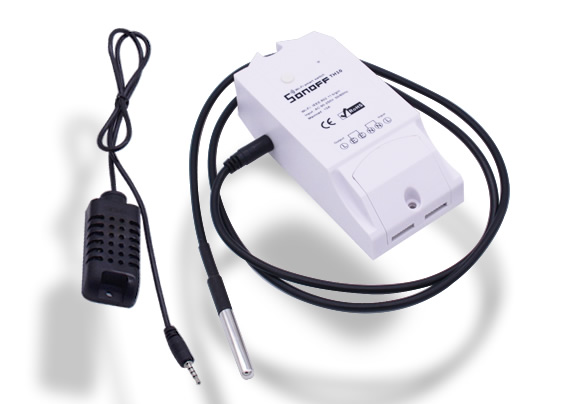
\includegraphics[width=0.33\textwidth]{./imagenes/teoria/TH1.jpg} }
\\

\subfloat[G1]
{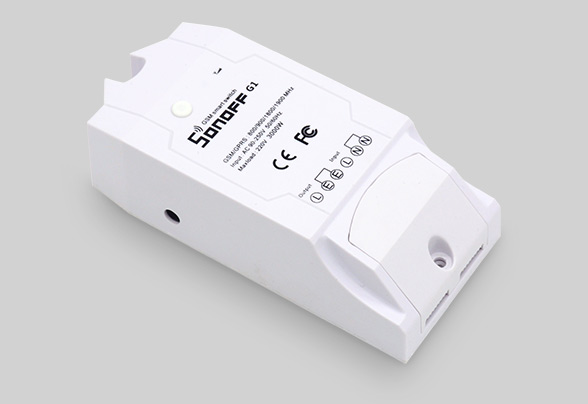
\includegraphics[width=0.33\textwidth]{./imagenes/teoria/G1.jpg}}
&
\subfloat[4CHPRO]{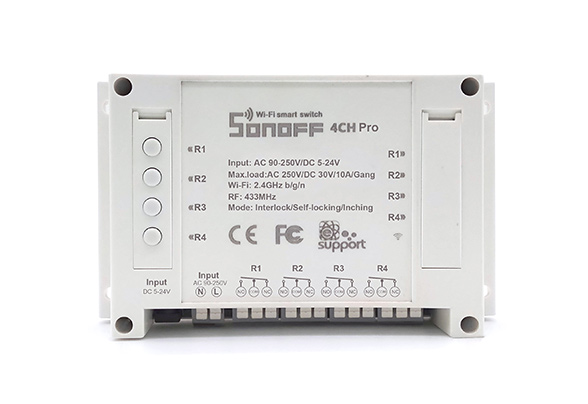
\includegraphics[width=0.33\textwidth]{./imagenes/teoria/4CHPRO.jpg} }
&
\subfloat[Pow R2]{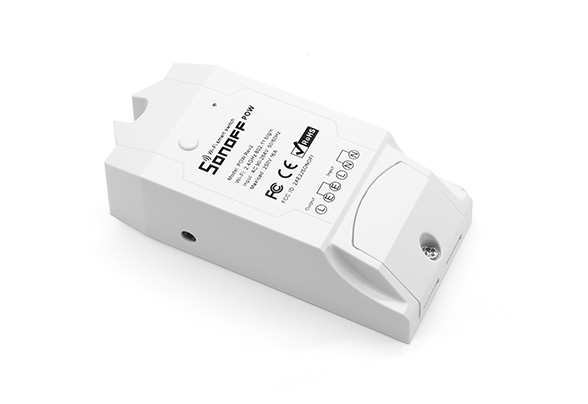
\includegraphics[width=0.33\textwidth]{./imagenes/teoria/POWR2.jpg} }
\\

\subfloat[Dual]
{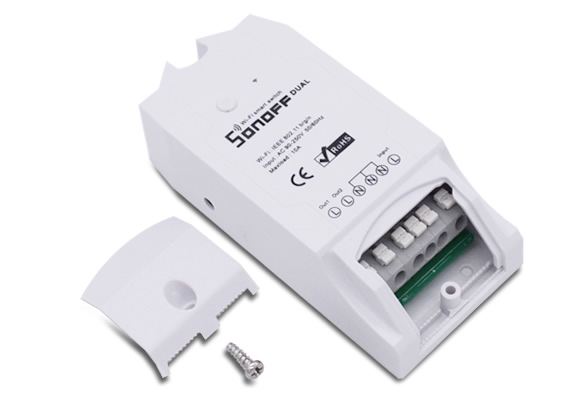
\includegraphics[width=0.33\textwidth]{./imagenes/teoria/DUAL.jpg}}
&
\subfloat[Pow]{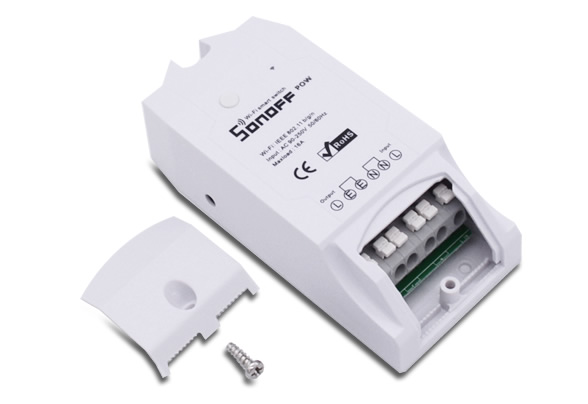
\includegraphics[width=0.33\textwidth]{./imagenes/teoria/POW.jpg} }
&
\subfloat[4CH]{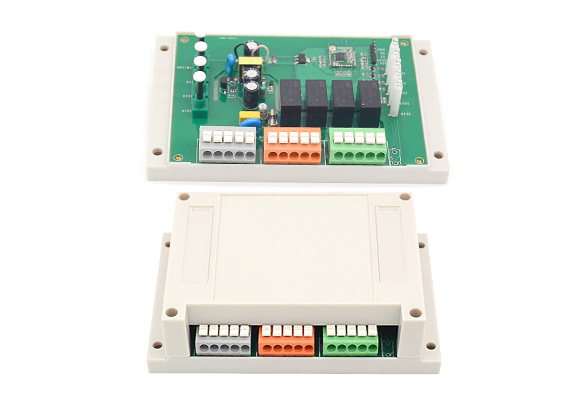
\includegraphics[width=0.33\textwidth]{./imagenes/teoria/4CH.jpg} }
\\

\end{tabular}
\caption{Componentes electrónicos Sonoff.}
\label{F:PRODUCTS}
\end{figure}


%%%------------------------------------------
\subsection{Reprogramación de los componentes Sonoff}
%%%------------------------------------------

Como se menciono anteriormente, una de las principales ventajas de estos componentes es que se pueden editar la configuración por defecto de los mismos. Estos componentes se pueden abrir y realizar la configuración de pines para conectar por comunicación serial haciendo uso de un módulo de conexión USB.

Una vez realizada está configuración, se puede editar usando el \textit{Arduino IDE}, el cual es un software de código abierto, que hace que sea fácil escribir código y subirlo a la tarjeta. Se ejecuta en Windows, Mac OS X y Linux. El entorno está escrito en Java y está basado en \textit{Processing} y otro software de código abierto. A la hora de programación tiene una sintaxis lingüística muy similar a la de C \cite{Arduino2018}. 

\begin{figure}[H]
\centering
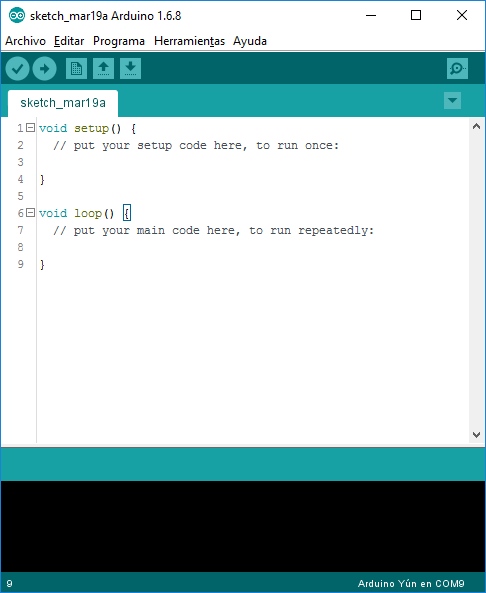
\includegraphics[width=0.8\textwidth]{./imagenes/teoria/ide.png} 
\caption{Interfaz del Arduino IDE \cite{Arduino2018}.}
\label{F:IDE}
\end{figure}



%%%------------------------------------------
\section{Interfaces de usuario}
%%%------------------------------------------

Las interfaces de usuario, son la parte de programa o aplicación que interactúa con un usuario para realizar tareas específicas.

Douglas Engelbart, además de inventor del ratón de ordenador, desarrolló la primera interfaz gráfica en los años 1960 en EE.UU. en los laboratorios de XEROX. Fue introducida posteriormente al público en las computadoras Apple Macintosh en 1984, y a las masas hasta 1993 con la primera versión popular del sistema operativo Windows 3.0

En la actualidad, el uso de interfaces de usuario se encuentra en diversas áreas debido a sus facilidad de interacción con el usuario, por lo que hoy día lo podemos ver en cualquier tipo de componentes, como celulares, microondas, cocinas, lavadoras, carros, televisores, aires acondicionados, radios, aviones, entre muchos otros ejemplos más. Por lo tanto, La historia reciente de la informática está indisolublemente unida a las interfaces gráficas, puesto que los sistemas operativos gráficos han ocasionado grandes consecuencias en la industria del software y del hardware \cite{Pavon2017}. Las interfaces de usuario se han divido en tres áreas fundamentales, las cuales son:

\begin{itemize}
\item \textbf{CLI} : La interfaz de línea de comandos (\textit{Command Line Interface}, por sus siglas en inglés), es un método que permite a los usuarios dar instrucciones a algún programa informático por medio de una línea de texto simple, actualmente conocido como Terminal o Bash.
\item \textbf{GUI} : La interfaz gráfica de usuario (\textit{Graphical User Interface}, por sus siglas en inglés)  es un método para facilitar la interacción del usuario con el ordenador o la computadora a través de la utilización de un conjunto de imágenes y objetos pictóricos (iconos, ventanas...) además de texto. Surge como evolución de la línea de comandos de los primeros sistemas operativos y es pieza fundamental en un entorno gráfico \cite{Pavon2017}.

\item \textbf{NUI} : La interfaz natural de usuario (\textit{Natural User Interface}, por sus siglas en inglés), según \cite{Pavon2017}, en este tipo el usuario interactúa con un sistema, aplicación, etcétera, sin utilizar sistemas de mando o dispositivos de entrada (como en las interfaces gráficas de usuarios, sería un ratón, teclado alfanumérico, lápiz óptico, panel táctil, joystick, etcétera), y en su lugar, se hace uso de movimientos gestuales del cuerpo o de alguna de sus partes tales como las manos, sirviendo de mando de control.
\end{itemize}

A continuación en la figura \ref{F:GUI}, se puede apreciar una imagen que ejemplifica de mejor manera esta clasificación.

\begin{figure}[H]
\centering
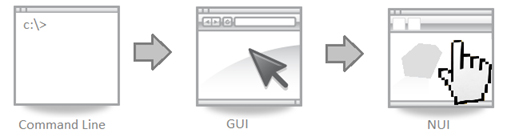
\includegraphics[width=\textwidth]{./imagenes/teoria/gui.jpg} 
\caption{Tipos generales de interfaces gráficas.}
\label{F:GUI}
\end{figure}

Para este proyecto, se hará especial énfasis a las GUI, ya que, es lo que  se desea diseñar en este proyecto, aunque en la actualidad la surgido una gran tendencia en el área de sistemas domóticos a usar interfaces de usuario tipo NUI, debido a que facilita el uso celulares y tablets. 

Debido al amplio uso de las GUI en tantas diversas áreas existen varios lenguajes de programación y herramientas para el diseño de interfaces gráficas, a continuación se presentan los principales:

\begin{itemize}
\item Python.
\item Glade.
\item Java (AWT  y Swing).
\item QT5.
\item Visual Basic.
\item WXWINDOWS.
\end{itemize}

Además existen varios principios que se usan para el diseño de interfaces gráficas de manera correcta, se manejan los siguientes conceptos:

\begin{itemize}
\item Sencilla
\item Flexible
\item Coherente
\item Autonomía
\item Percepción del color
\item Legibilidad 
\end{itemize}

%%%------------------------------------------
\subsection{Desarrollo de interfaces con QT5}
%%%------------------------------------------

Según \cite{QT52018}, se dice Qt es un framework multiplataforma orientado a objetos ampliamente usado para desarrollar programas (software) que utilicen interfaz gráfica de usuario, así como también diferentes tipos de herramientas para la línea de comandos y consolas para servidores que no necesitan una interfaz gráfica de usuario.

En 1991, Haavard Nord y Eirik Chambe-Eng, inician el desarrollo de QT, desde ese entonces a formado parte de la plataforma usada por grandes compañías a nivel mundial para el diseño de interfaces, empezando desde el 2001 con Nokia. En Marzo 2011, se publicó una versión, en el cuál se inicia la compatibilidad con Android, iOS, Linux y la plataforma de Windows. En la figura \ref{F:qt5}, se muestra el logo que representa la marca. 

\begin{figure}[H]
\centering

\includegraphics[width=0.3\textwidth]{./imagenes/teoria/qt5.jpg} 
\caption{Logo de la marca comercial QT5. \cite{QT52018}}
\label{F:qt5}
\end{figure}

Entre sus principales características se encuentra que:

\begin{itemize}
\item Es de software libre y código abierto.
\item El lenguaje de programación es C++, de forma nativa, adicionalmente puede ser utilizado en varios otros lenguajes de programación a través de \textit{bindings} \footnote{\textbf{Bindings}: es una adaptación de una biblioteca para ser usada en un lenguaje de programación distinto de aquel en el que ha sido escrita.}.
\item Usa un lenguaje declarativo, por lo que se describe el aspecto de los elementos y se centra en interfaces gráficas.
\item Una de las ventajas de usar esta herramienta, es que debido a su auge en los últimos años, se encuentran disponibles en línea varios manuales, foros y tutoriales que ayudan al uso de la plataforma. 
\end{itemize}

Es ampliamente usado por la industria de sistemas embedidos y empresas como: Agencia Espacial Europea, DreamWorks, Lucasfilm, Panasonic, Philips, Samsung, Siemens AG, Volvo, Walt Disney Animation Studios, Blizzard Entertainment, Electronic Arts, AMD, Research In Motion, HP, entre otros; hacen uso de este software para el desarrollo de las interfaces gráficas para sus productos. Para el caso del diseño de interfaces para sistemas domóticos usando esta herramienta, en la actualidad ya se han realizado proyectos de esta índole, por lo que en este proyecto se propone usar manuales de referencia. En la figura \ref{F:homeqt5}, se muestra un ejemplo del diseño de una interfaz con este software.

\begin{figure}[H]
\centering
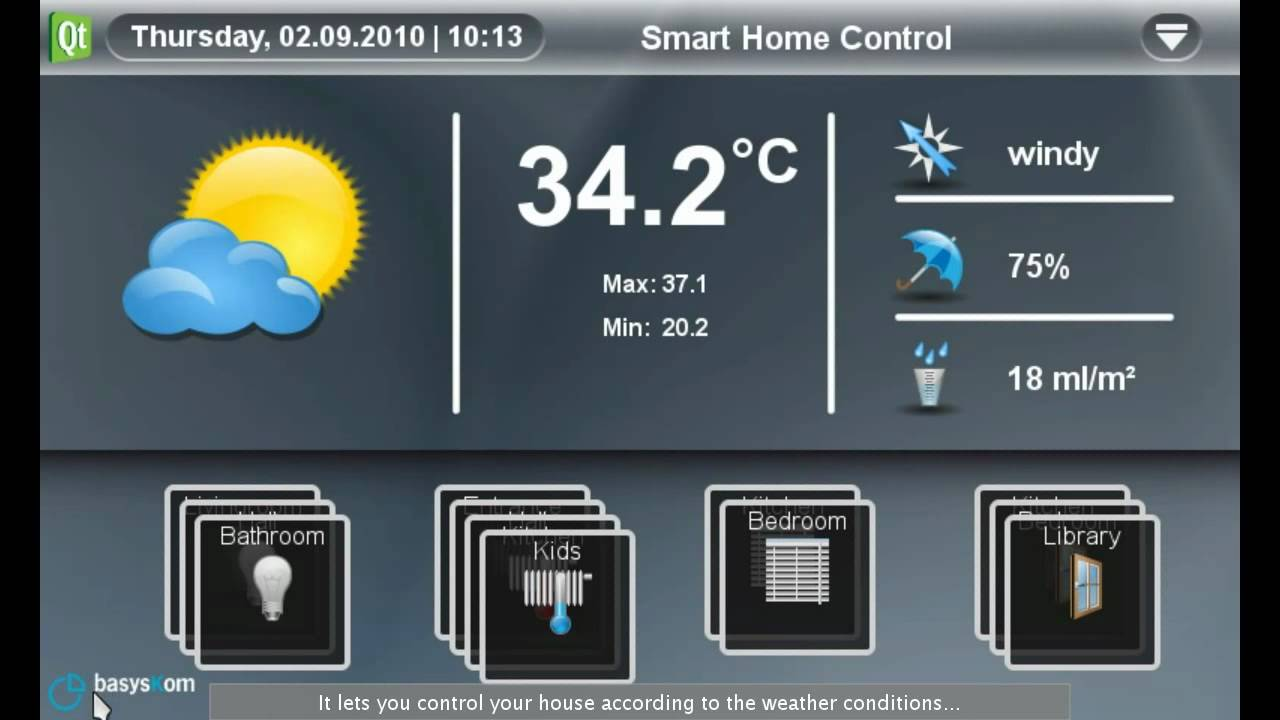
\includegraphics[width=0.8\textwidth]{./imagenes/teoria/homeqt.jpg} 
\caption{Ejemplo de interfaz para sistemas domótico diseñado con QT5. \cite{QT52018}}
\label{F:homeqt5}
\end{figure}



